%\documentclass[handout]{beamer}
\documentclass[compress]{beamer}

\usepackage[T1]{fontenc}
\usepackage[utf8]{inputenc}
\usepackage[american]{babel}

\usepackage{csquotes}
\usepackage[style=apa, backend=biber]{biblatex}
\DeclareLanguageMapping{american}{american-apa}

\usepackage{pifont}
\usepackage{threeparttable}
\usepackage{subcaption}
\usepackage{tikz-qtree}
\usepackage{tikz}
\usetikzlibrary{positioning,arrows.meta}
\usepackage{multicol}
\usepackage{booktabs}
\usepackage{graphicx}
\usepackage{neuralnetwork}
\usepackage{hyperref}
\usepackage{xcolor}
\usepackage{fvextra}
\usepackage[newfloat]{minted}

\addbibresource{../resources/literature.bib}
\graphicspath{{../resources/pictures/}}

\hypersetup{
  pdfborder={0 0 0},
  colorlinks=true,
  pdfauthor={Anne Kroon, Saurabh Khanna},
  pdftitle={Computational Communication Science 2}
}

\usetheme[
  block=fill,
  subsectionpage=progressbar,
  sectionpage=progressbar
]{metropolis}

\definecolor{Purple}{HTML}{911146}
\definecolor{Orange}{HTML}{CF4A30}

\setbeamercolor{alerted text}{fg=Orange}
\setbeamercolor{frametitle}{bg=Purple,fg=white}
\setbeamercolor{structure}{fg=Purple}
\setbeamercolor{normal text}{bg=white,fg=black}

\setbeamercovered{
  still covered={\opaqueness<1->{5}},
  again covered={\opaqueness<1->{100}}
}

\setbeamersize{text margin left=12pt,text margin right=12pt}

\setbeamertemplate{section page}[progressbar]
\setbeamertemplate{subsection page}[progressbar]

\setbeamertemplate{itemize item}{\color{Purple}$\bullet$}

\setbeamerfont{frametitle}{size=\Large,series=\bfseries}
\setbeamerfont{framesubtitle}{size=\normalsize}
\setbeamerfont{normal text}{size=\small}
\setbeamerfont{itemize/enumerate body}{size=\small}
\setbeamerfont{itemize/enumerate subbody}{size=\small}
\setbeamerfont{block title}{size=\large,series=\bfseries}

\renewcommand*{\bibfont}{\tiny}

\makeatletter
\setbeamertemplate{headline}{%
    \begin{beamercolorbox}[colsep=1.5pt]{upper separation line head}
    \end{beamercolorbox}
    \begin{beamercolorbox}{section in head/foot}
        \vskip2pt\insertnavigation{\paperwidth}\vskip2pt
    \end{beamercolorbox}
    \begin{beamercolorbox}[colsep=1.5pt]{lower separation line head}
    \end{beamercolorbox}
}
\makeatother

\usemintedstyle{colorful}
\setminted{
  breaklines=true,
  fontsize=\scriptsize,
  bgcolor=gray!5
}

\newcommand{\question}[1]{
    \begin{frame}[plain]
        \begin{columns}
            \column{.4\textwidth}
            \makebox[\columnwidth]{%
                
\includegraphics[width=\columnwidth,height=\paperheight,keepaspectratio]{mannetje.png}}
            \column{.6\textwidth}
            \large
            \textcolor{Orange}{\textbf{\emph{#1}}}
        \end{columns}
    \end{frame}
}

\newcommand{\instruction}[1]{\emph{\textcolor{gray}{[#1]}}}

\title[CCS2]{\textbf{Computational Communication Science 2} \\
Week 3 -- Lecture\\
\emph{Text Similarity and Recommender Systems}}

\author[Anne Kroon]{Anne Kroon \\ \footnotesize{a.c.kroon@uva.nl}}

\date{April 13, 2026}

\institute[Digital Society Minor]{Digital Society Minor, University of Amsterdam}

\begin{document}

\begin{frame}{}
  \titlepage
\end{frame}

\begin{frame}{Today}
  \begin{tiny}
    \tableofcontents
  \end{tiny}
\end{frame}

\question{Everything clear from last week?}

%------------------------------------------------------------
\begin{frame}{Where are we in the course?}
\centering
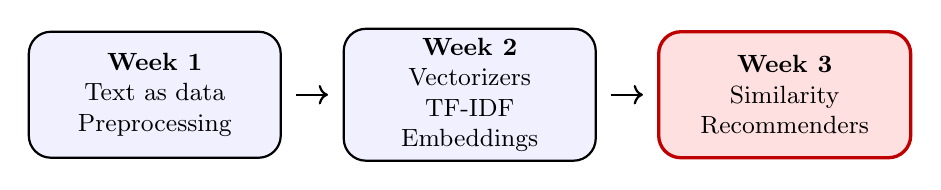
\begin{tikzpicture}[
    every node/.style={font=\small},
    stage/.style={
        draw,
        rounded corners=8pt,
        minimum width=3.2cm,
        minimum height=1.6cm,
        align=center,
        thick,
        fill=blue!6
    },
    highlight/.style={
        draw,
        rounded corners=8pt,
        minimum width=3.2cm,
        minimum height=1.6cm,
        align=center,
        very thick,
        draw=red!75!black,
        fill=red!12
    }
]

\node[stage] (w1) at (0,0) {\textbf{Week 1}\\Text as data\\Preprocessing};
\node[stage] (w2) at (4,0) {\textbf{Week 2}\\Vectorizers\\TF-IDF\\Embeddings};
\node[highlight] (w3) at (8,0) {\textbf{Week 3}\\Similarity\\Recommenders};

\draw[->, thick] (1.8,0) -- (2.2,0);
\draw[->, thick] (5.8,0) -- (6.2,0);

\end{tikzpicture}

\vspace{0.6cm}

\begin{alertblock}{This week}
We move from \textbf{representing text} to \textbf{comparing texts} and using similarity for recommendations.
\end{alertblock}

\end{frame}

%------------------------------------------------------------
\begin{frame}{Main points from last week}
  \begin{alertblock}{By now, you should know how to:}
    \begin{itemize}[<+>]
      \item clean and preprocess textual data;
      \item represent text as vectors;
      \item understand the difference between Count, TF-IDF, and embeddings.
    \end{itemize}
  \end{alertblock}
\end{frame}

%------------------------------------------------------------
\begin{frame}{Linking back: how do we analyse text?}
\begin{block}{Two approaches}
\begin{itemize}
\item<1-> \textbf{Top-down} --- define categories in advance \\
(e.g., dictionary-based sentiment analysis)
\item<2-> \textbf{Bottom-up} --- let patterns emerge from the data \\
(e.g., similarity, embeddings, topic models)
\end{itemize}
\end{block}

\pause

\begin{alertblock}{Why this matters today}
Cosine similarity and embeddings are \textbf{bottom-up methods}: we do not define categories in advance --- we compare texts directly.
\end{alertblock}
\end{frame}

%------------------------------------------------------------
\section{Cosine Similarity}

\begin{frame}{Why text similarity matters}
  \begin{block}{Core idea}
    Once text has been represented as vectors, we can compare documents numerically.
  \end{block}
  \pause
  \begin{exampleblock}{Why this is useful}
    \begin{itemize}[<+>]
      \item compare news articles, speeches, or reviews
      \item detect overlap between texts
      \item track change over time
      \item build recommender systems
    \end{itemize}
  \end{exampleblock}
\end{frame}

\begin{frame}{Cosine Similarity}
  \begin{block}{What is cosine similarity?}
    A measure of how similar two documents are, regardless of their length.
  \end{block}
  \pause
  \begin{exampleblock}{Applications in Communication Science}
    \begin{itemize}[<+>]
      \item Measuring \emph{linguistic alignment} of romantic couples over time \parencite{Brinberg2021}
      \item Measuring agenda overlap between public opinion and political speech \parencite{Hager2020}
    \end{itemize}
  \end{exampleblock}
\end{frame}

\begin{frame}{Cosine Similarity: the formula}
  $$
    \text{similarity} = \cos(\theta) =
    \frac{\mathbf{A} \cdot \mathbf{B}}{\|\mathbf{A}\|\|\mathbf{B}\|}
  $$
  \pause
  \begin{itemize}[<+>]
    \item Measures the cosine of the angle between two vectors.
    \item \textbf{0} = no overlap in direction
    \item \textbf{1} = identical direction
    \item Higher score = more similar
  \end{itemize}
\end{frame}

\begin{frame}{Cosine Similarity: visualised}
  \makebox[\columnwidth]{%
    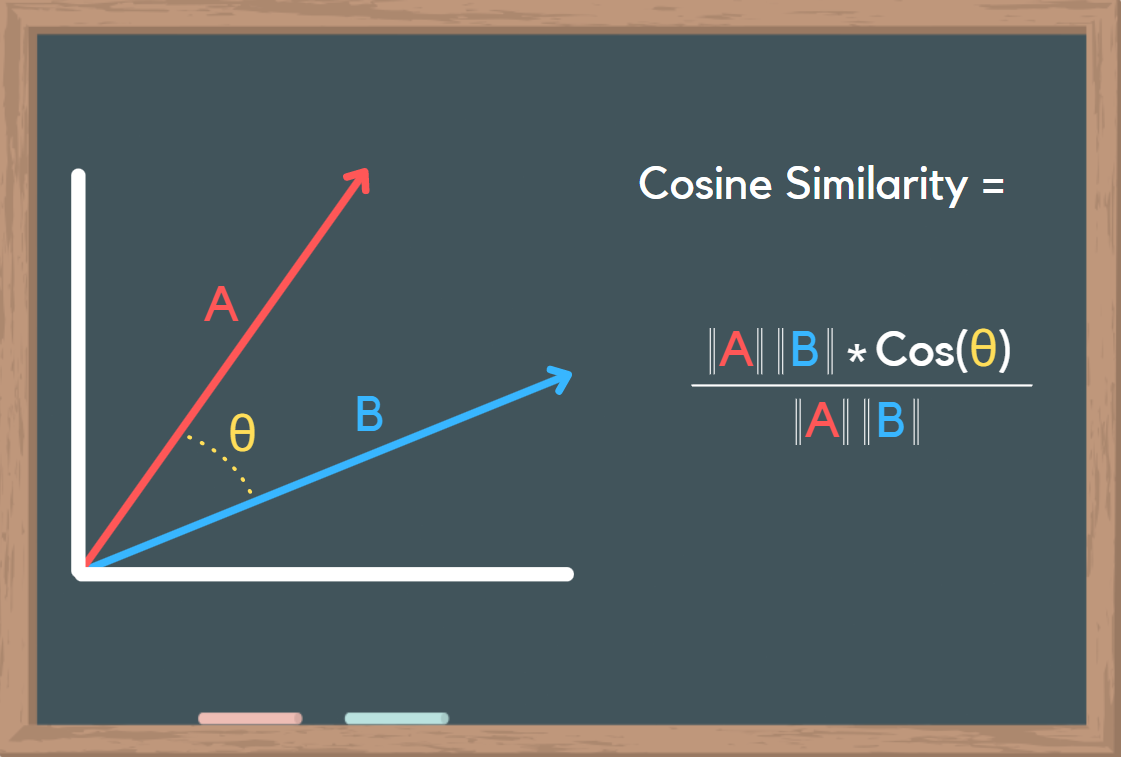
\includegraphics[width=\columnwidth,height=\paperheight,keepaspectratio]{cosine_angle.png}}
  \vspace{0.3em}
  {\tiny Source: \url{https://towardsdatascience.com/what-is-cosine-similarity-how-to-compare-text-and-images-in-python-d2bb6e411ef0}}
\end{frame}

\begin{frame}[fragile]{Step 1: vectorize the documents}
\begin{minted}[linenos]{python}
from sklearn.feature_extraction.text import CountVectorizer
import pandas as pd

doc1 = "when i eat breakfast i usually drink some tea"
doc2 = "i like my tea with my breakfast"
doc3 = "she likes cereal and coffee"

vec = CountVectorizer(stop_words="english")
count_matrix = vec.fit_transform([doc1, doc2, doc3])

print(pd.DataFrame(
    count_matrix.toarray(),
    columns=vec.get_feature_names_out()
).to_string())
\end{minted}
\pause
\begin{minted}{text}
   breakfast  cereal  coffee  drink  eat  like  likes  tea  usually
0          1       0       0      1    1     0      0    1        1
1          1       0       0      0    0     1      0    1        0
2          0       1       1      0    0     0      1    0        0
\end{minted}
\end{frame}

\begin{frame}{Cosine similarity: intuition}
  \begin{block}{What is happening?}
    \begin{itemize}[<+>]
      \item Each document is converted into a vector of numbers.
      \item Each number shows whether or how often a word appears.
      \item We compare vectors instead of sentences directly.
    \end{itemize}
  \end{block}
  \pause
  \begin{exampleblock}{Key idea}
    Documents with similar word patterns get a higher similarity score.
  \end{exampleblock}
\end{frame}

\begin{frame}[fragile]{Step 2: compute cosine similarity}
\begin{minted}[linenos]{python}
from sklearn.metrics.pairwise import cosine_similarity

cos_sim = cosine_similarity(count_matrix)
print(cos_sim)
\end{minted}
\pause
\begin{minted}{text}
[[1.         0.51639778 0.        ]
 [0.51639778 1.         0.        ]
 [0.         0.         1.        ]]
\end{minted}
\end{frame}

\begin{frame}{How to read this matrix}
  \begin{block}{Interpretation}
    \begin{itemize}[<+>]
      \item The matrix compares every document with every other document.
      \item The diagonal is always \textbf{1}: each document is identical to itself.
      \item \textbf{0.52}: doc1 and doc2 are somewhat similar.
      \item \textbf{0}: doc3 has no exact word overlap with the others.
    \end{itemize}
  \end{block}
\end{frame}

\begin{frame}{Interpreting cosine similarity}
  \begin{block}{What do the values mean?}
    \begin{itemize}[<+>]
      \item \textbf{1.0} = identical in this representation
      \item \textbf{higher values} = more overlap in words
      \item \textbf{0.0} = no overlap in this representation
    \end{itemize}
  \end{block}
  \pause
  \begin{alertblock}{Important}
    Cosine similarity is \textbf{relative}: a score is meaningful only compared to other texts in your dataset.
  \end{alertblock}
\end{frame}

\begin{frame}[fragile]{Mini play-around exercise}
\begin{minted}[linenos]{python}
from sklearn.feature_extraction.text import CountVectorizer
from sklearn.metrics.pairwise import cosine_similarity

docs = [
    "I drink tea at breakfast",
    "Tea is part of my breakfast routine",
    "I eat cereal and drink coffee"
]

vec = CountVectorizer(stop_words="english")
X = vec.fit_transform(docs)

print(vec.get_feature_names_out())
print(cosine_similarity(X))
\end{minted}

\pause

\begin{alertblock}{Try this}
Change one sentence or add a fourth sentence. What happens to the similarity scores?
\end{alertblock}
\end{frame}

\begin{frame}{What can you do with cosine similarity?}
  \begin{block}{Practical applications}
    \begin{itemize}[<+>]
      \item compare news articles, speeches, movies, song lyrics
      \item detect overlap between texts
      \item build simple search or recommender systems
    \end{itemize}
  \end{block}
\end{frame}

\begin{frame}{Example: movie similarity by genre}
  \makebox[\linewidth]{%
    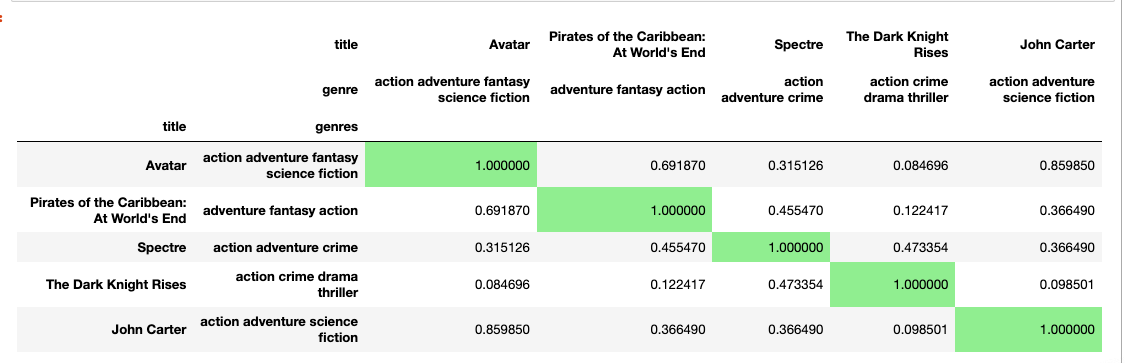
\includegraphics[width=\columnwidth,height=\paperheight,keepaspectratio]{cosine_sim.png}}
\end{frame}

\begin{frame}[fragile]{What about documents with no words in common?}
\begin{minted}[linenos]{python}
print(cosine_similarity(count_matrix))
\end{minted}
\pause
\begin{minted}{text}
[[1.         0.51639778 0.        ]
 [0.51639778 1.         0.        ]
 [0.         0.         1.        ]]
\end{minted}
\pause
\begin{alertblock}{Problem}
Doc3 (\textit{``she likes cereal and coffee''}) gets a score of \textbf{0} with the others --- even though the texts are about related breakfast concepts.
\end{alertblock}
\end{frame}

\begin{frame}{Things to consider when using cosine similarity}
  \begin{block}{Design choices}
    \begin{itemize}[<+>]
      \item What kind of overlap are you interested in?
      \item How should you preprocess? Stopwords, stemming, n-grams?
      \item Should you use raw counts or TF-IDF?
    \end{itemize}
  \end{block}
  \pause
  \begin{alertblock}{Key limitation}
    Cosine similarity based on bag-of-words relies on \textbf{exact word overlap}. Synonyms and paraphrases are largely invisible.
  \end{alertblock}
\end{frame}

%------------------------------------------------------------
\section{Semantic Similarity}

\begin{frame}{Beyond exact overlap}
  \begin{block}{Why do we need another method?}
    \begin{itemize}[<+>]
      \item Two texts can mean similar things even if they do not use the same words.
      \item Basic cosine similarity does not capture this well.
      \item We therefore need a way to compare \textbf{meaning}, not just matching words.
    \end{itemize}
  \end{block}
\end{frame}

\begin{frame}{What are word embeddings?}
  \begin{block}{Core idea}
    \begin{itemize}[<+>]
      \item Word embeddings are vector representations of words.
      \item Words with similar meanings end up close together in vector space.
      \item This allows us to compare texts based on meaning.
    \end{itemize}
  \end{block}
\end{frame}

\begin{frame}{The key idea}
  \begin{exampleblock}{Instead of exact overlap}
    \begin{itemize}[<+>]
      \item \textit{tea} and \textit{coffee} are different words
      \item \textit{breakfast} and \textit{cereal} are different words
      \item but they are still semantically related
    \end{itemize}
  \end{exampleblock}
  \pause
  \begin{alertblock}{So what changes?}
    We compare documents using embeddings, so semantically related texts can still get a higher similarity score.
  \end{alertblock}
\end{frame}

\begin{frame}[fragile]{A simple embedding-based example}
\begin{minted}[linenos]{python}
import spacy

nlp = spacy.load("en_core_web_md")

doc1 = "when i eat breakfast i usually drink some tea"
doc2 = "i like my tea with my breakfast"
doc3 = "she likes cereal and coffee"

d1 = nlp(doc1)
d2 = nlp(doc2)
d3 = nlp(doc3)

print(f"doc1 <-> doc2: {d1.similarity(d2):.2f}")
print(f"doc1 <-> doc3: {d1.similarity(d3):.2f}")
print(f"doc2 <-> doc3: {d2.similarity(d3):.2f}")
\end{minted}
\end{frame}

\begin{frame}{How to interpret this}
  \begin{block}{What is happening here?}
    \begin{itemize}[<+>]
      \item spaCy represents each text as a vector using pre-trained embeddings.
      \item We then compare those text vectors.
      \item Unlike bag-of-words cosine, this can pick up on semantic relatedness.
    \end{itemize}
  \end{block}
  \pause
  \begin{exampleblock}{Expected result}
    The similarity between doc1/doc3 and doc2/doc3 should now be \textbf{above zero}, because the texts are about related breakfast concepts.
  \end{exampleblock}
\end{frame}

\begin{frame}[fragile]{Which movie is more similar?}
  \begin{block}{Goal}
    Find the best match for the query
  \end{block}
\begin{minted}{python}
query  = "A young wizard discovers he has magical powers"
movie1 = "A boy learns magic at a boarding school"
movie2 = "A detective investigates a murder case"

q = nlp(query)
m1 = nlp(movie1)
m2 = nlp(movie2)
\end{minted}
  \pause
  \begin{alertblock}{Think first}
    Which movie should be more similar?
  \end{alertblock}
\end{frame}

\begin{frame}[fragile]{Result}
\begin{minted}{python}
print("Wizard vs magic school:", q.similarity(m1))
print("Wizard vs detective:", q.similarity(m2))
\end{minted}
  \pause
  \begin{block}{Output (example)}
    \begin{itemize}
      \item Wizard vs magic school: \textbf{0.72}
      \item Wizard vs detective: \textbf{0.18}
    \end{itemize}
  \end{block}
  \pause
  \begin{alertblock}{Takeaway}
    The model prefers the magic-related movie because it captures \textbf{meaning}, not just exact word overlap.
  \end{alertblock}
\end{frame}

%------------------------------------------------------------
\section[RecSys]{Recommender Systems}

\begin{frame}{}
  \makebox[\linewidth]{%
    
\includegraphics[width=\columnwidth,height=\paperheight,keepaspectratio]{social_media.jpeg}}
\end{frame}

\begin{frame}{Recommender Systems in Communication Science}
  \begin{block}{Why do they matter?}
    \begin{enumerate}[<+>]
      \item \alert{Political communication \& journalism} \\
      Personalised news diets can affect diversity and democracy \parencite{Moller2018, Locherbach2018}

      \item \alert{Organisational communication} \\
      Hiring and recruitment applications

      \item \alert{Persuasive communication} \\
      Tailored health interventions \parencite{Kim2019}

      \item \alert{Entertainment communication} \\
      Movie and content recommendations
    \end{enumerate}
  \end{block}
\end{frame}

\begin{frame}{How do recommender systems learn?}
  \begin{block}{Sources of information}
    \begin{enumerate}[<+>]
      \item \alert{Explicit preferences} \\
      Ratings, likes, reviews

      \item \alert{Implicit preferences} \\
      Clicks, watch time, purchase history

      \item \alert{Content} \\
      Similarity between items
    \end{enumerate}
  \end{block}
\end{frame}

\begin{frame}{Types of recommender systems}
  \begin{block}{Three main approaches \parencite{Wieland2021, Locherbach2018, Moller2018}}
    \begin{enumerate}[<+>]
      \item Knowledge-based recommender systems
      \item Content-based recommender systems
      \item Collaborative filtering
    \end{enumerate}
  \end{block}
  \pause
  \begin{alertblock}{Focus today}
    \begin{itemize}
      \item Knowledge-based = based on what the user asks for
      \item Content-based = based on similarity between items
    \end{itemize}
  \end{alertblock}
\end{frame}

%------------------------------------------------------------
\section[Knowledge-based RS]{Knowledge-based Recommender Systems}

\begin{frame}{Knowledge-based recommender systems}
  \begin{block}{When do we use them?}
    \begin{itemize}[<+>]
      \item Useful when you have \textbf{no user ratings}: the cold start problem
      \item Recommendations are based on explicit user input
      \item Typical use case: real estate, where purchases are rare
    \end{itemize}
  \end{block}
\end{frame}

\begin{frame}{}
  \makebox[\linewidth]{%
    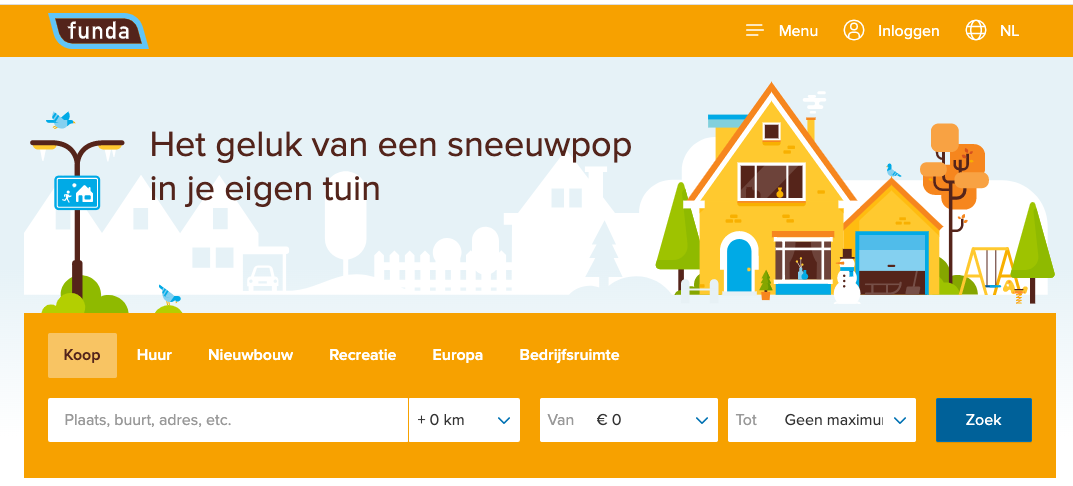
\includegraphics[width=\columnwidth,height=\paperheight,keepaspectratio]{funda}}
\end{frame}

\begin{frame}{Use case: IMDb dataset}
  \makebox[\linewidth]{%
    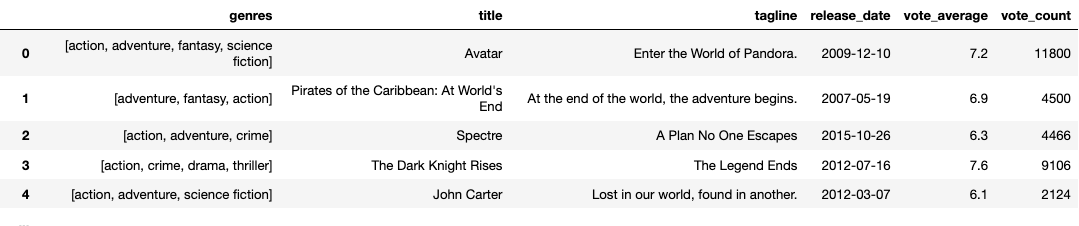
\includegraphics[width=\columnwidth,height=\paperheight,keepaspectratio]{data}}
\end{frame}

\question{What variables would you use in a knowledge-based recommender system?}

\begin{frame}[fragile]{Getting user input in Python}
Without a front-end, we can use Python's built-in \texttt{input()} function:
\pause
\begin{minted}[linenos]{python}
print("What is your favorite movie genre?")
genre = input()
\end{minted}
\pause
\begin{minted}{text}
What is your favorite movie genre?
[user types here]
\end{minted}
\end{frame}

\begin{frame}[fragile]{Improving a knowledge-based recommender}
  \begin{block}{Make recommendations more relevant}
    \begin{itemize}[<+>]
      \item Think about what extra information can improve relevance.
      \item For example, sort by average rating to show stronger items first.
    \end{itemize}
  \end{block}
\pause
\begin{minted}[linenos]{python}
recommended = movies.sort_values("vote_average", ascending=False)
\end{minted}
\end{frame}

%------------------------------------------------------------
\section[Content-based RS]{Content-based Recommender Systems}

\begin{frame}{Content-based recommender systems}
  \begin{block}{How do they work?}
    \begin{itemize}[<+>]
      \item Recommend items based on similarity between item features
      \item Features can include genre, plot, tags, director, or location
      \item Text similarity is often a key ingredient
    \end{itemize}
  \end{block}
\end{frame}

\begin{frame}{Example: content-based recommendation}
  \makebox[\linewidth]{%
    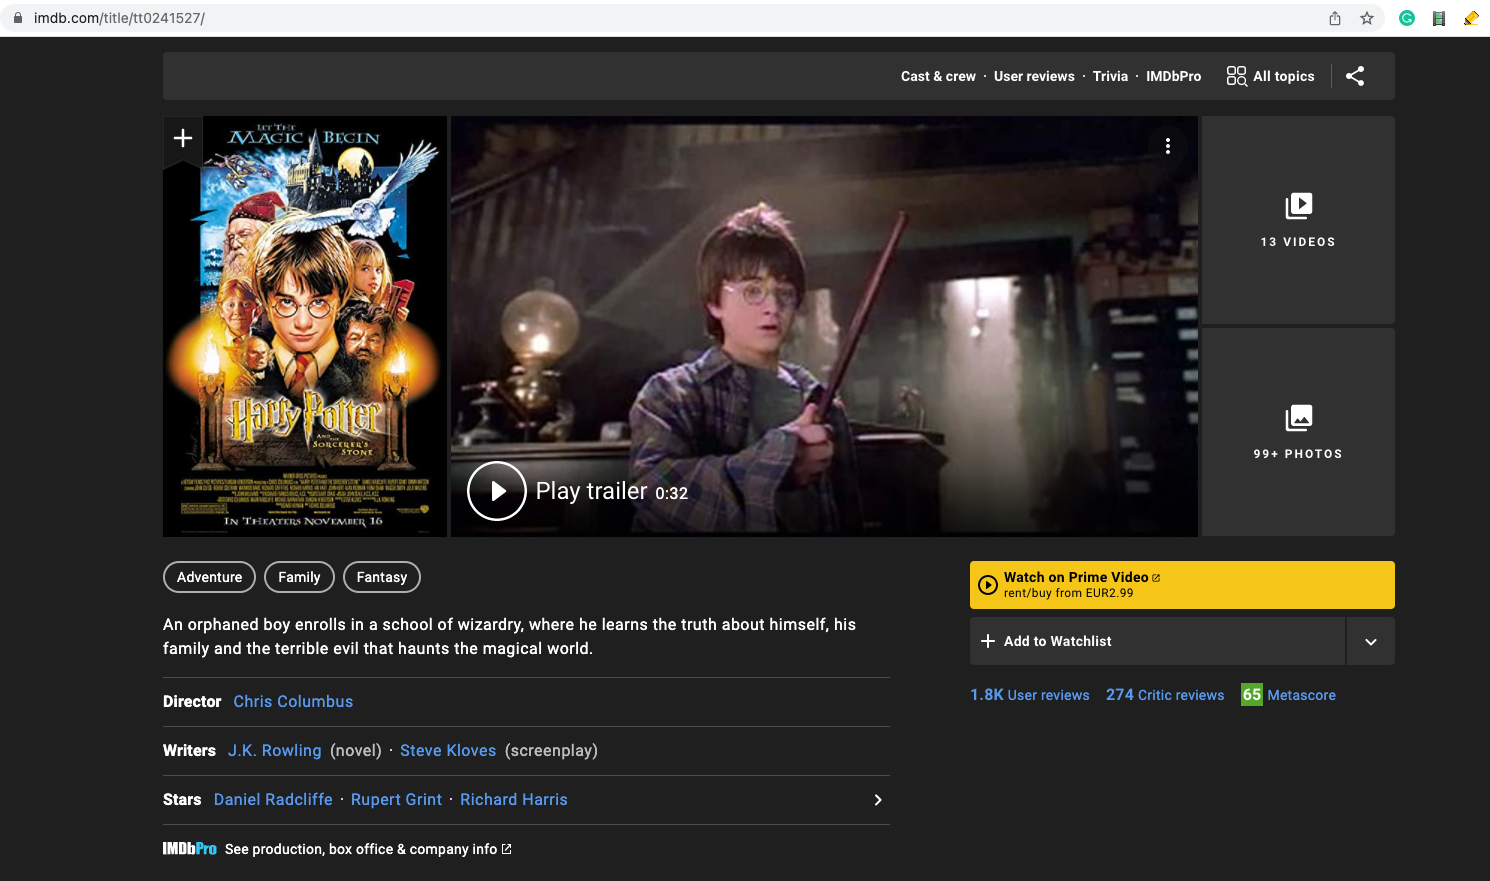
\includegraphics[width=\columnwidth,height=\paperheight,keepaspectratio]{harry1.png}}
\end{frame}

\begin{frame}{Example: content-based recommendation}
  \makebox[\linewidth]{%
    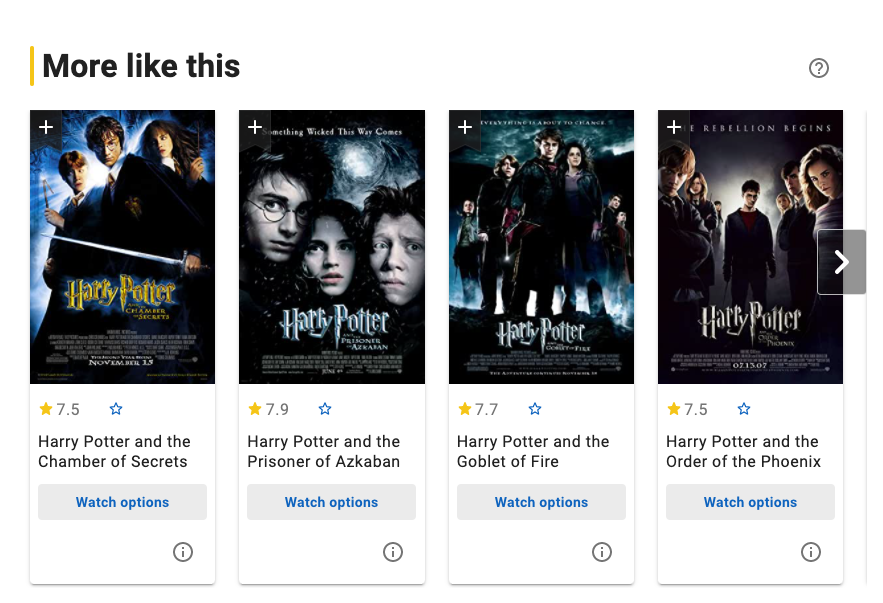
\includegraphics[width=\columnwidth,height=\paperheight,keepaspectratio]{harry2.png}}
\end{frame}

\begin{frame}{Use case: IMDb dataset}
Which attributes could you use to estimate similarity between movies?
  \makebox[\linewidth]{%
    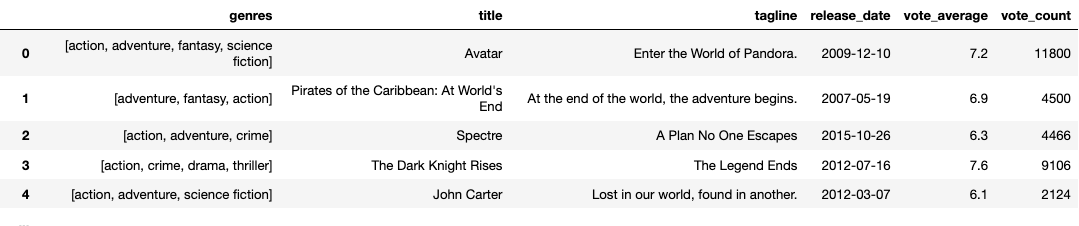
\includegraphics[width=\columnwidth,height=\paperheight,keepaspectratio]{data}}
\end{frame}

\begin{frame}{Similarity between movies}
  \only<1>{\makebox[\linewidth]{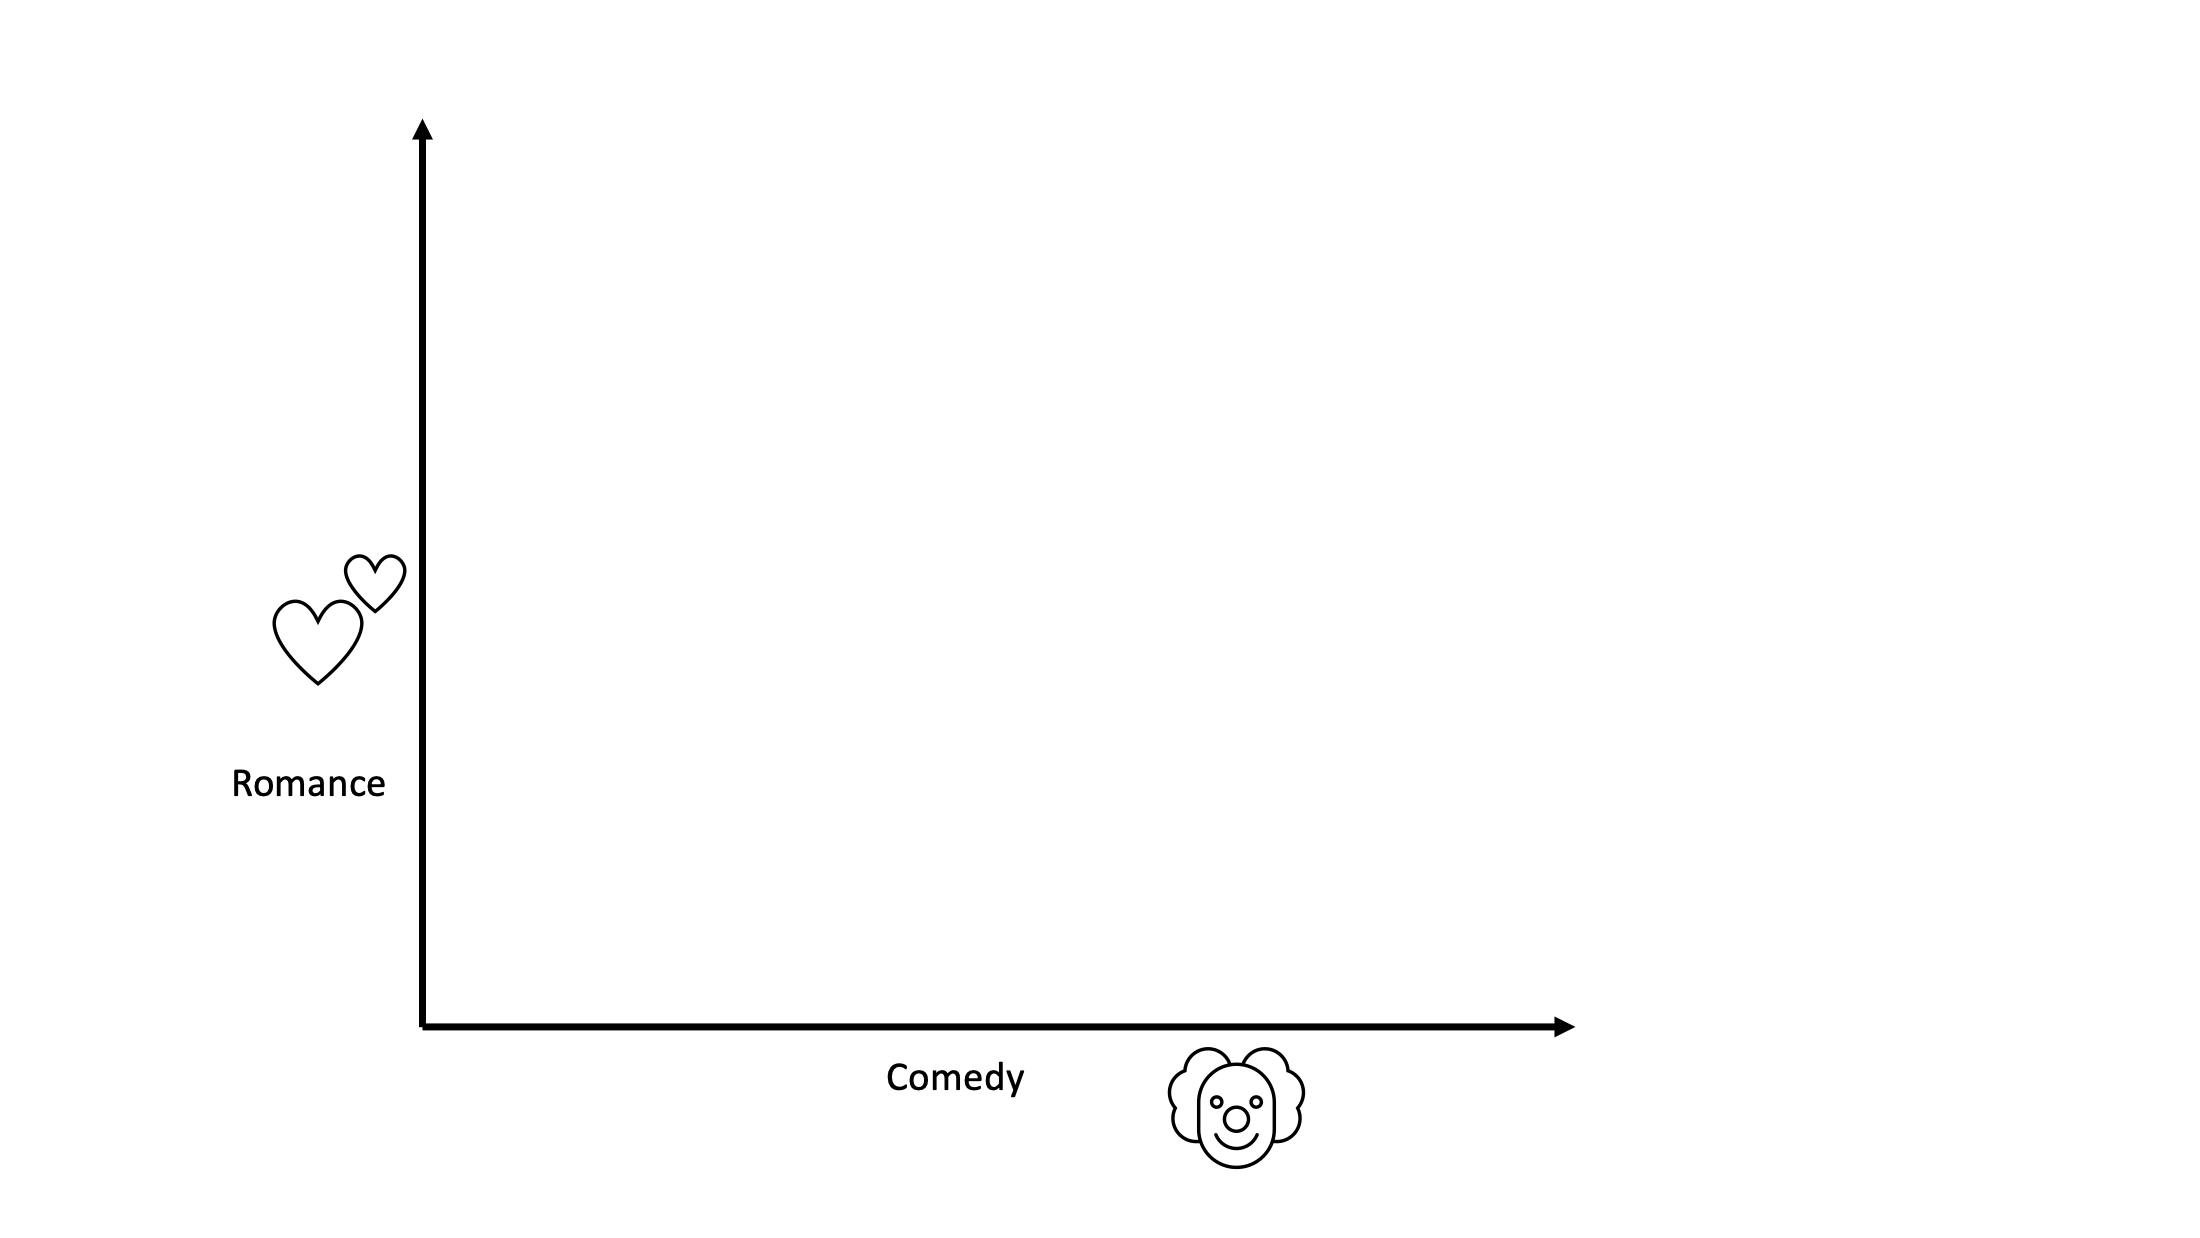
\includegraphics[width=\columnwidth,height=\paperheight,keepaspectratio]{Slide1.png}}}
  \only<2>{\makebox[\linewidth]{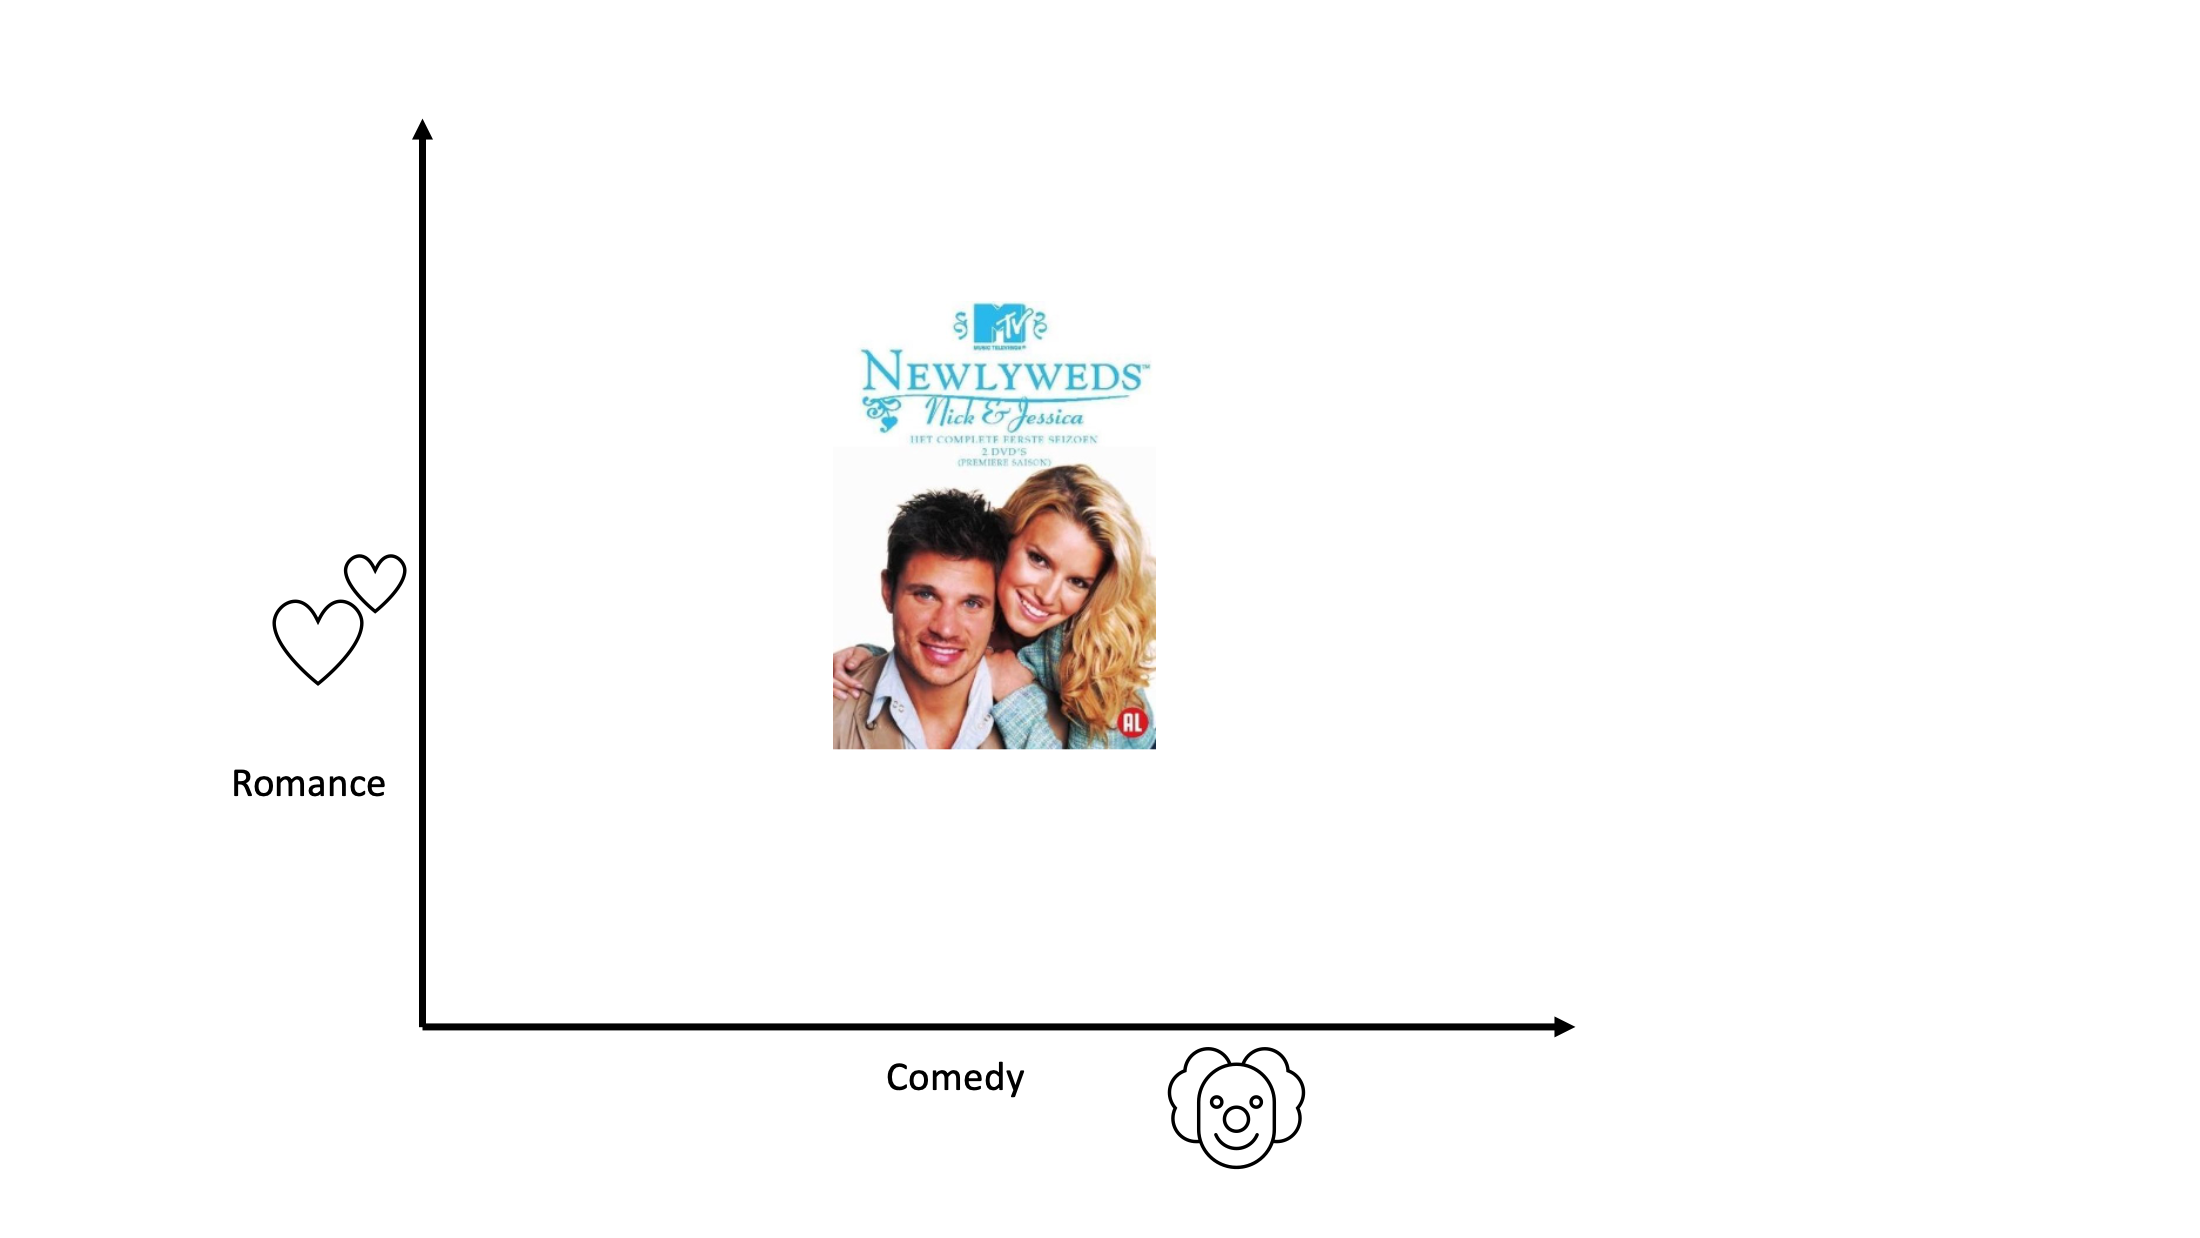
\includegraphics[width=\columnwidth,height=\paperheight,keepaspectratio]{Slide2.png}}}
  \only<3>{\makebox[\linewidth]{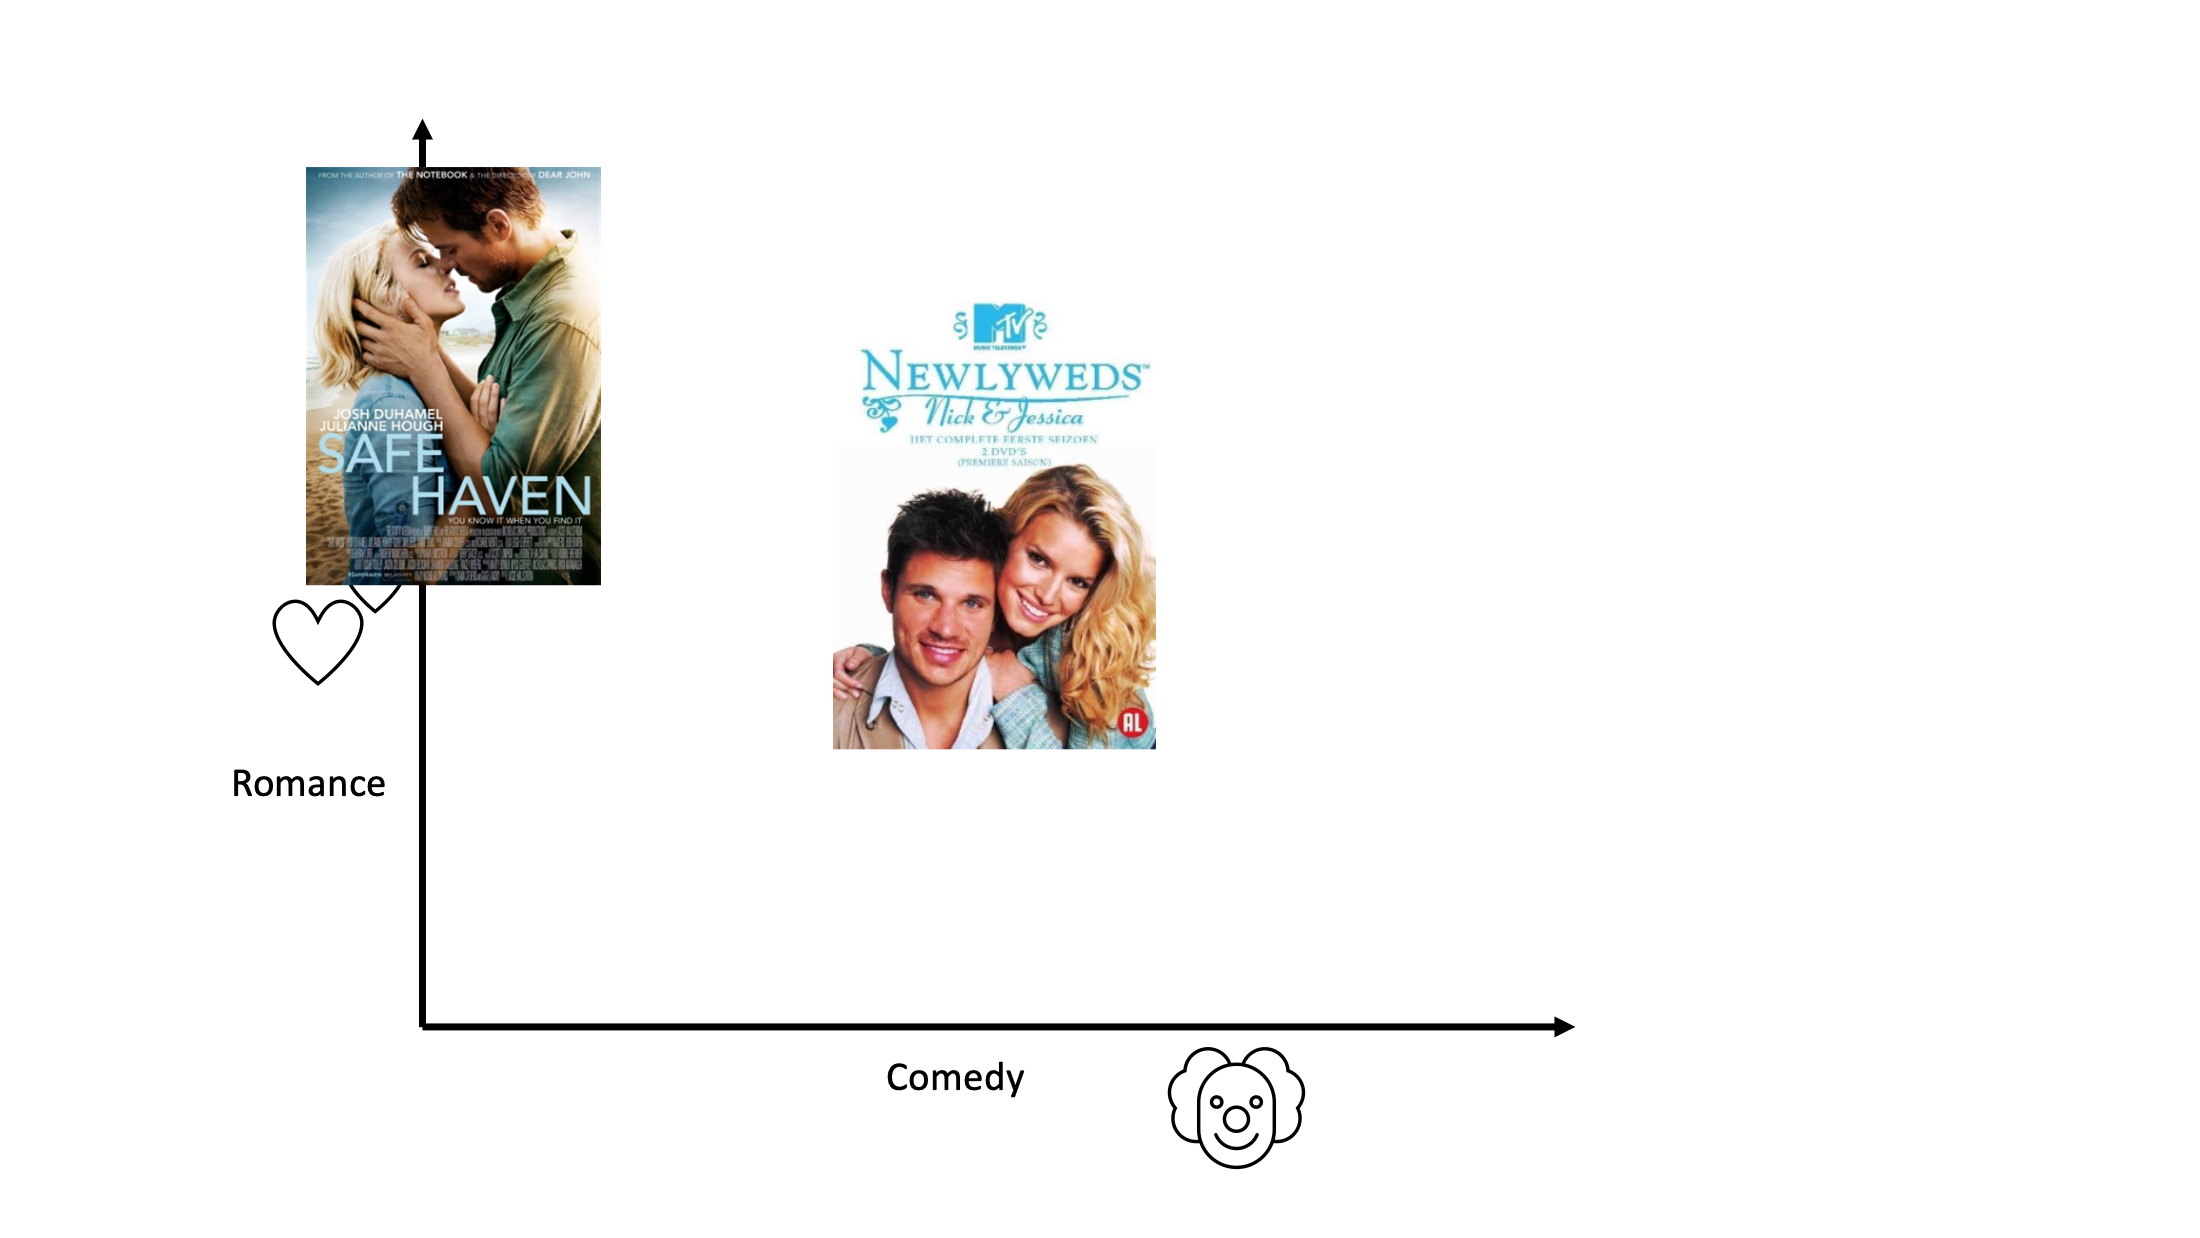
\includegraphics[width=\columnwidth,height=\paperheight,keepaspectratio]{Slide3.png}}}
  \only<4>{\makebox[\linewidth]{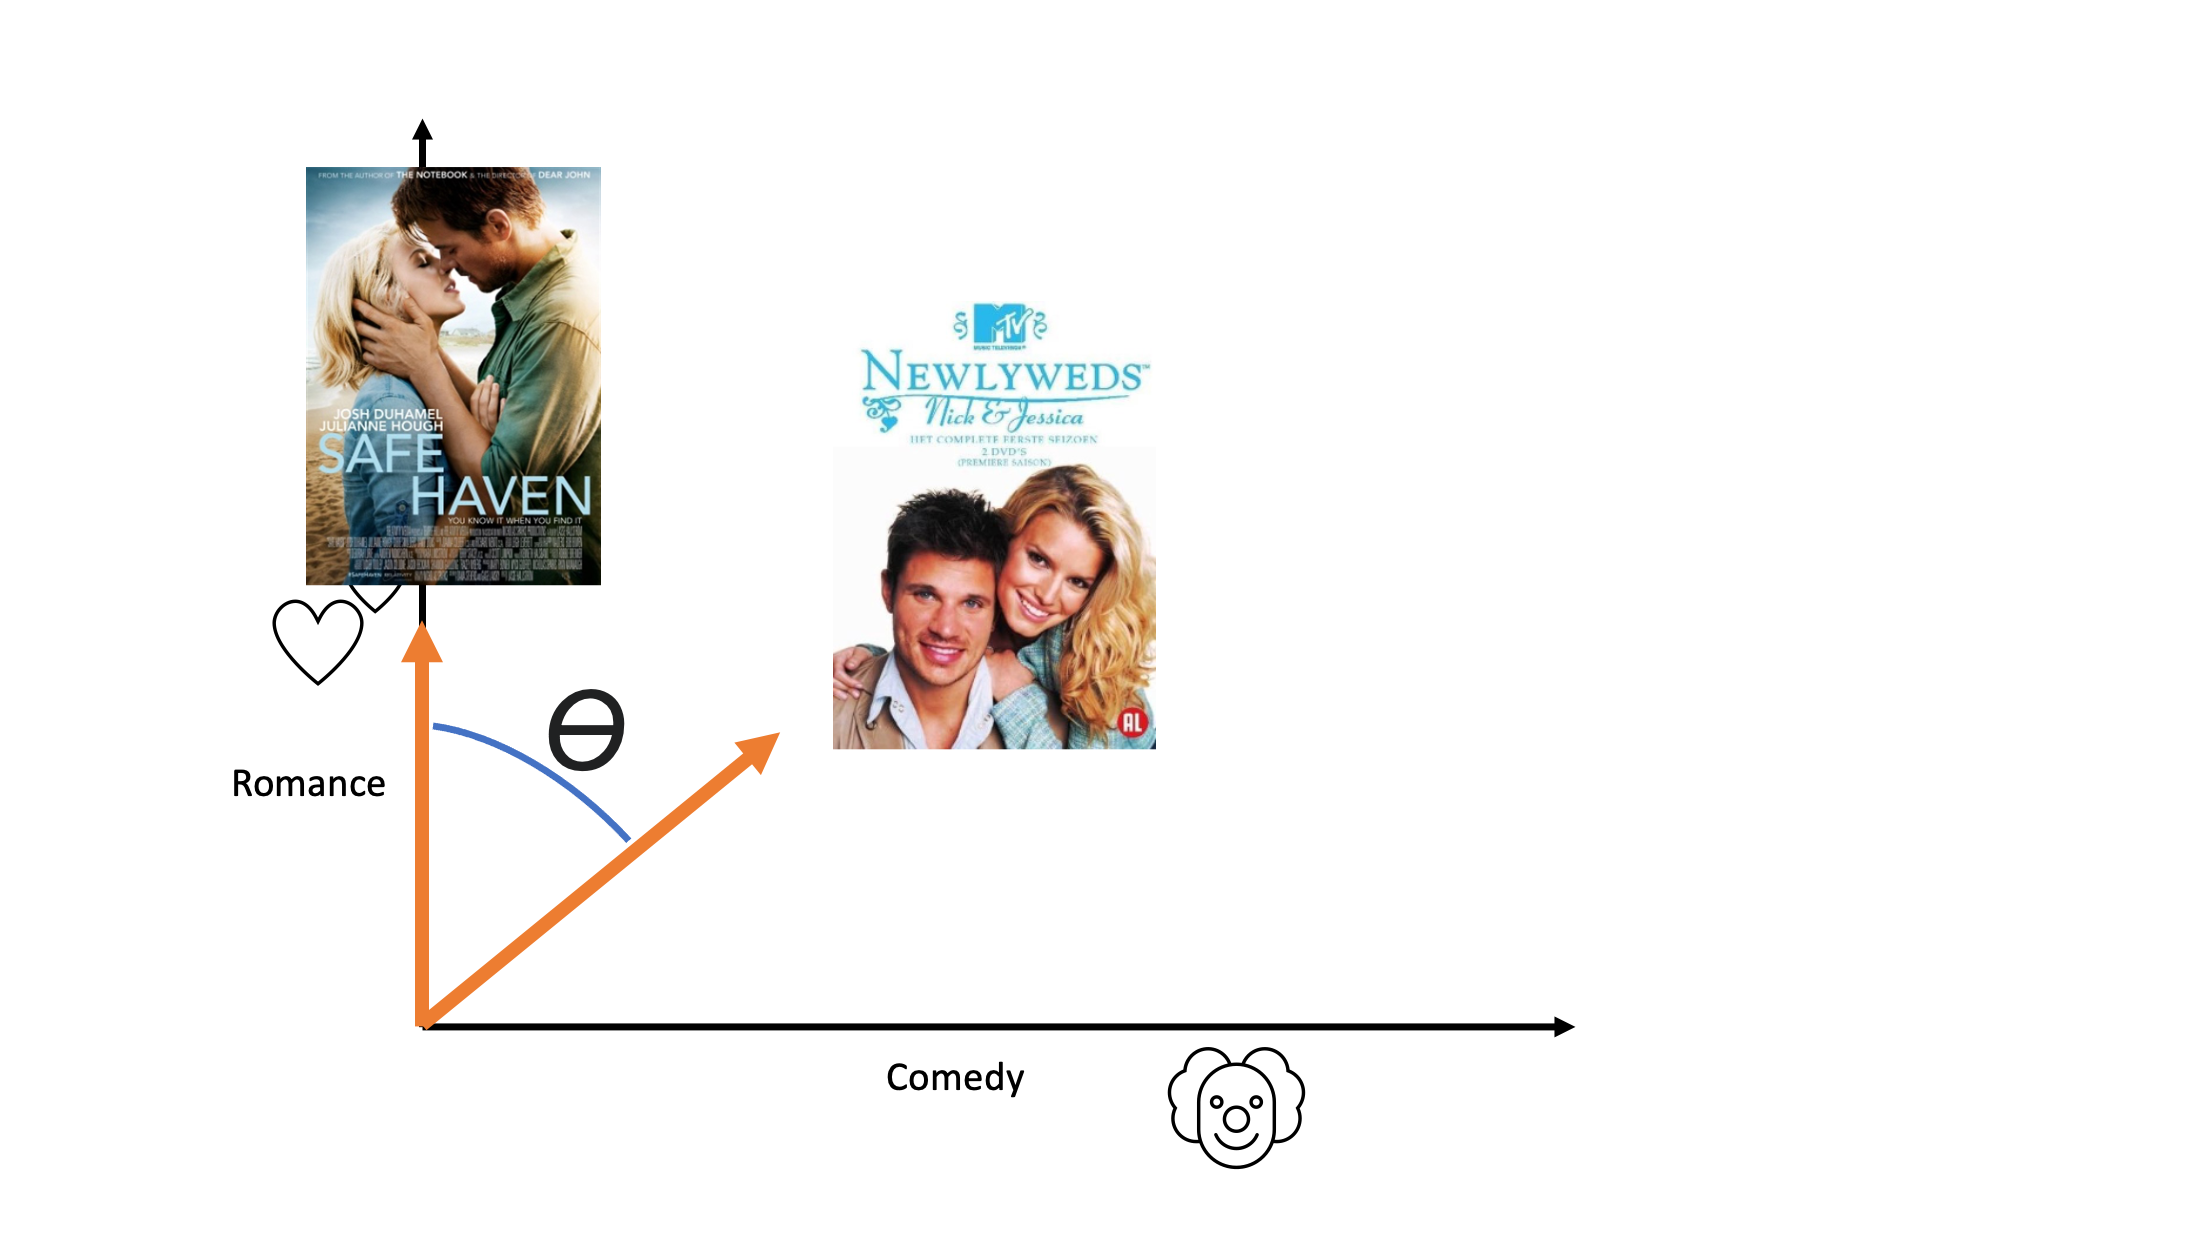
\includegraphics[width=\columnwidth,height=\paperheight,keepaspectratio]{Slide4.png}}}
  \only<5>{\makebox[\linewidth]{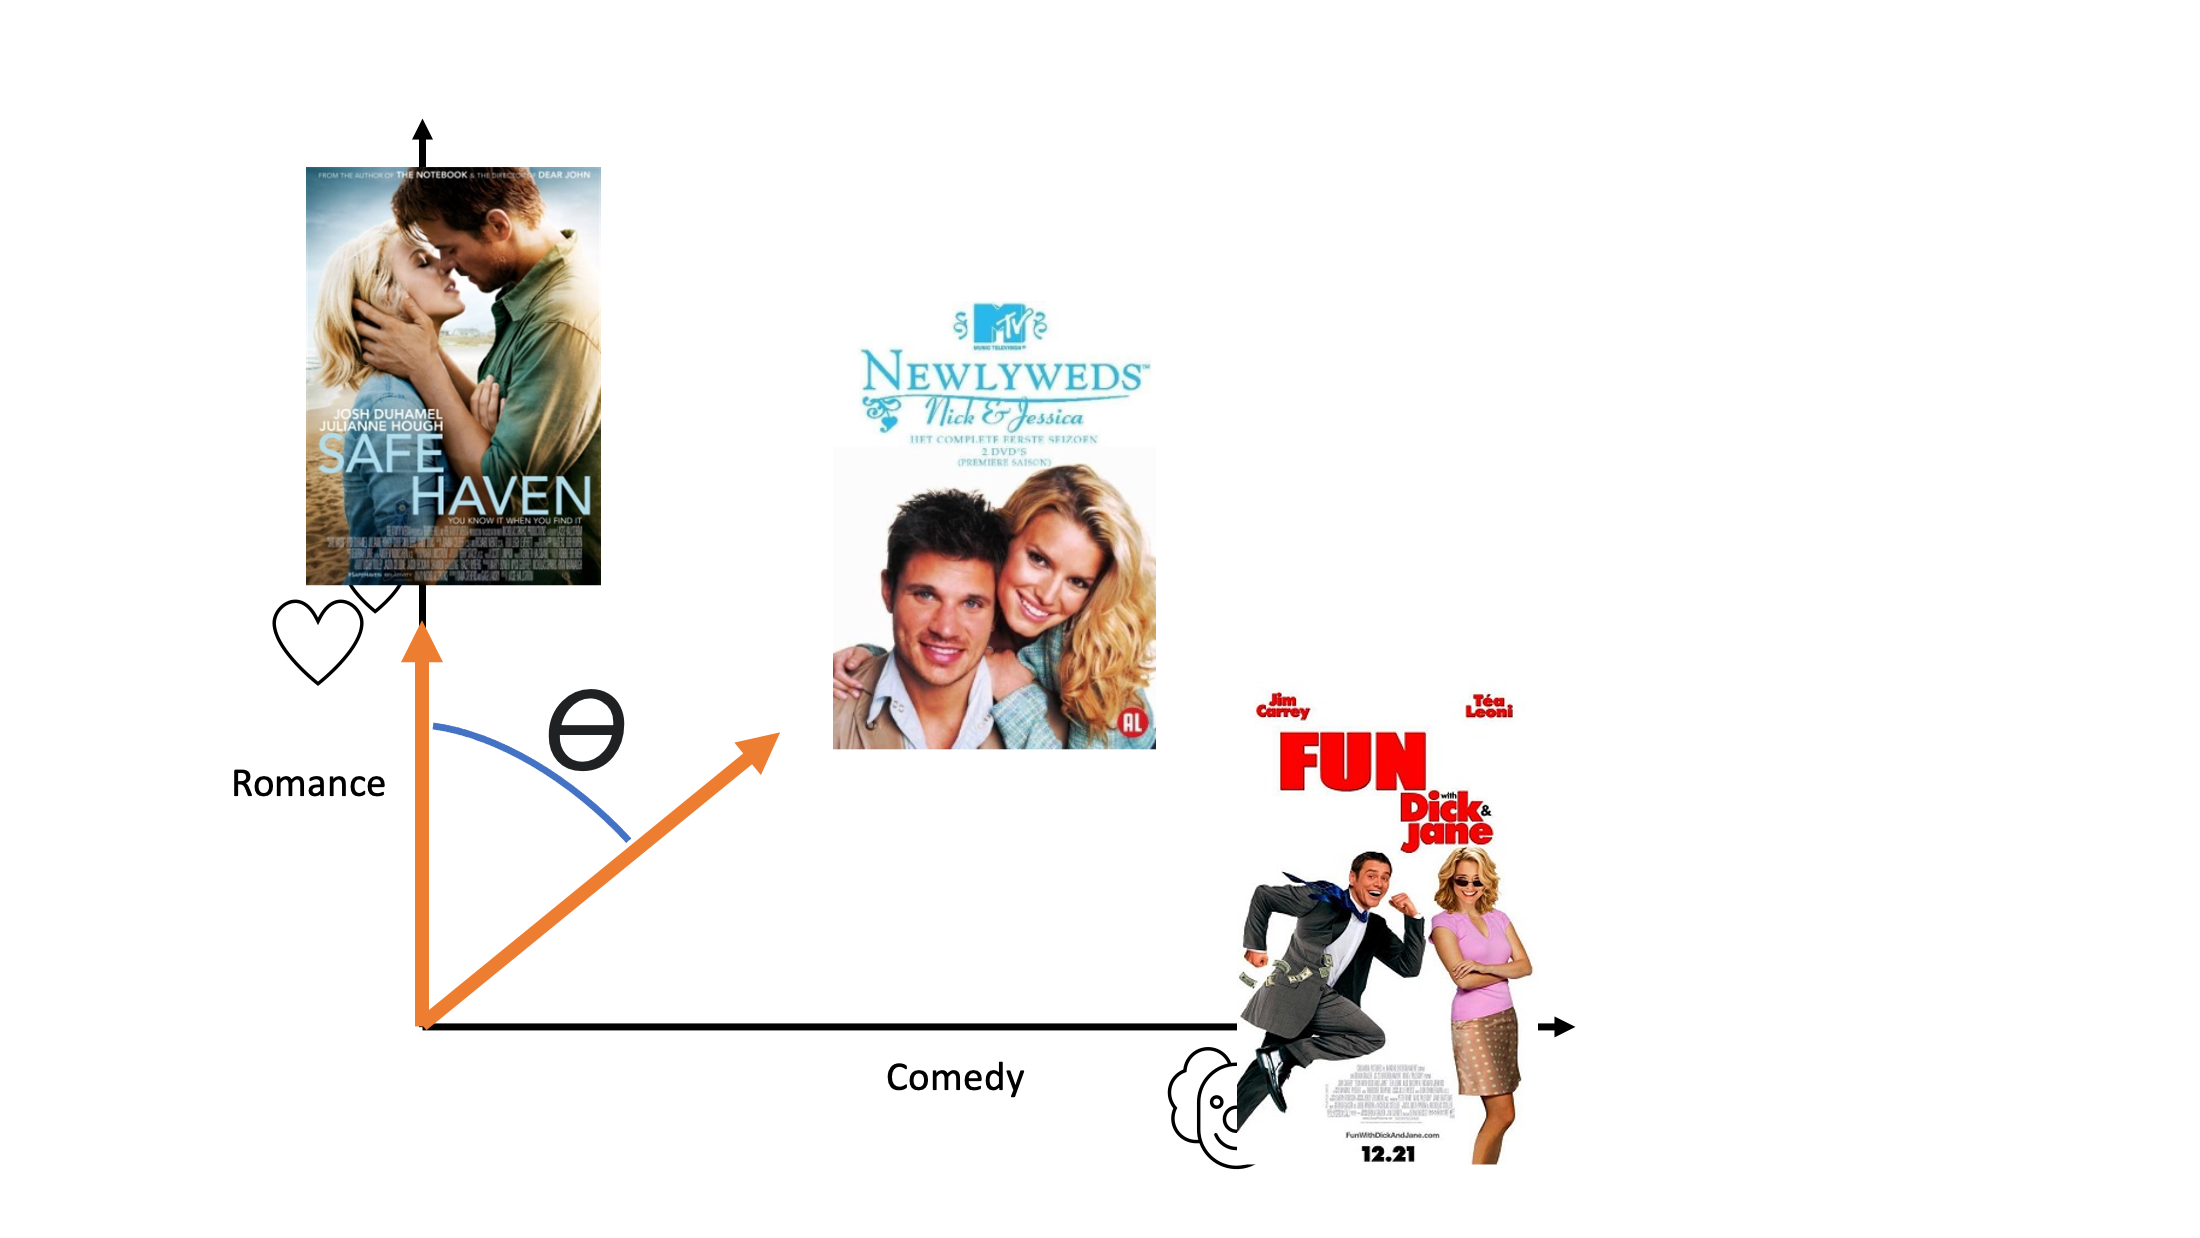
\includegraphics[width=\columnwidth,height=\paperheight,keepaspectratio]{Slide5.png}}}
\end{frame}

\begin{frame}[fragile]{Step 1: create a toy dataset}
\begin{minted}[linenos]{python}
data = data.sample(6)
print(data[["title", "genres"]])
\end{minted}
\pause
  \makebox[\linewidth]{%
    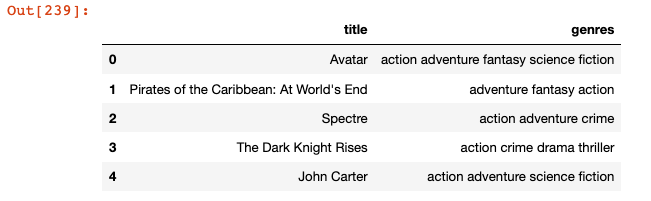
\includegraphics[width=\columnwidth,height=\paperheight,keepaspectratio]{toy}}
\end{frame}

\begin{frame}[fragile]{Step 2: vectorize the genre column}
\begin{minted}[linenos]{python}
from sklearn.feature_extraction.text import TfidfVectorizer

tfidf = TfidfVectorizer(stop_words="english")
tfidf_matrix = tfidf.fit_transform(data["genres"])
\end{minted}
\pause
\begin{alertblock}{Note}
We use TF-IDF here, but CountVectorizer could also be a valid choice depending on your goal.
\end{alertblock}
\end{frame}

\begin{frame}[fragile]{Step 3: calculate cosine similarity}
\begin{minted}[linenos]{python}
from sklearn.metrics.pairwise import cosine_similarity

sim = cosine_similarity(tfidf_matrix)
print(sim)
\end{minted}
\pause
\begin{minted}{text}
[[1.         0.34503493 0.         0.         0.40824829 0.        ]
 [0.34503493 1.         0.16581288 0.         0.28171984 0.29130219]
 [0.         0.16581288 1.         0.25964992 0.         0.56921261]
 [0.         0.         0.25964992 1.         0.44115109 0.4561563 ]
 [0.40824829 0.28171984 0.         0.44115109 1.         0.        ]
 [0.         0.29130219 0.56921261 0.4561563  0.         1.        ]]
\end{minted}
\small{Each cell is the similarity score between two movies.}
\end{frame}

\begin{frame}[plain]
  \makebox[\linewidth]{%
    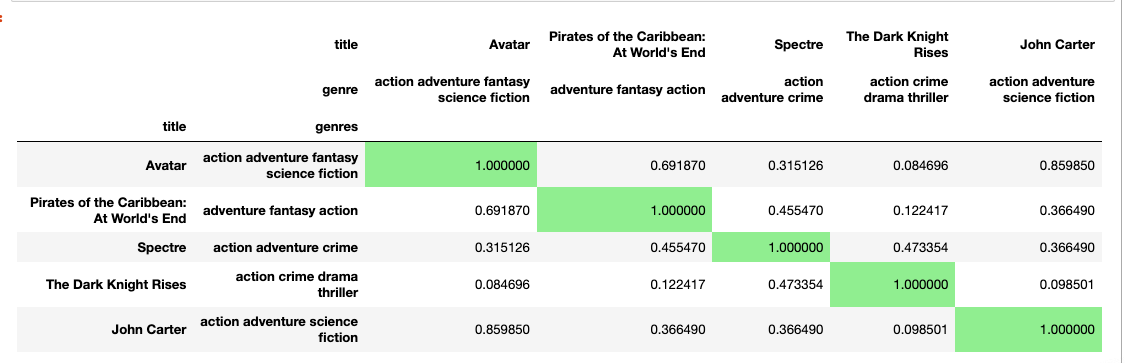
\includegraphics[width=\columnwidth,height=\paperheight,keepaspectratio]{cosine_sim}}
  \pause
  Users who like \textit{Avatar} may also enjoy \textit{John Carter}.
\end{frame}

\question{Can we automate this? Can we automatically find the most similar movie?}

\begin{frame}{From similarity matrix to recommendations}
  \begin{block}{The idea}
    \begin{itemize}[<+>]
      \item Combine multiple features into a single text representation
      \item Compute similarity across all movies
      \item For a given movie, rank the others by similarity score
      \item Return the top matches
    \end{itemize}
  \end{block}
  \pause
  \begin{exampleblock}{In the tutorial notebook}
    You will implement this step by step: combining features, computing similarity, and retrieving the top-$k$ most similar movies.\\
    \vspace{0.3em}
    {\small \url{https://github.com/uva-cw-ccs2/2526s2/blob/master/week03/exercise-tutorial/build_a_recommender_WALKTHROUGH.ipynb}}
  \end{exampleblock}
\end{frame}

\begin{frame}{Building blocks of content-based recommender systems}
  \begin{block}{Feature engineering matters}
    \begin{itemize}[<+>]
      \item What attributes do you include? Genre, plot, tags, director?
      \item You can also create your own features, for example topic scores from LDA.
    \end{itemize}
  \end{block}
  \pause
  \begin{block}{Ways to measure item similarity}
    \begin{enumerate}[<+>]
      \item Cosine similarity
      \item Embedding-based similarity
      \item LDA topic scores
    \end{enumerate}
  \end{block}
\end{frame}

\begin{frame}{Pros and cons of content-based systems}
  \begin{exampleblock}{Benefits}
    \begin{itemize}[<+>]
      \item Can work without any user rating data
      \item Often used as a component in larger systems
    \end{itemize}
  \end{exampleblock}
  \pause
  \begin{alertblock}{Drawbacks}
    \begin{itemize}[<+>]
      \item Only recommends items similar to what the user already knows
      \item Does not use community data
    \end{itemize}
  \end{alertblock}
\end{frame}

%------------------------------------------------------------
\section[Collaborative RS]{Collaborative Recommender Systems}

\begin{frame}{Collaborative filtering}
  \begin{block}{What is it?}
    \begin{itemize}[<+>]
      \item Tries to overcome the limitations of content-based systems
      \item Uses community data to give relevant and sometimes surprising recommendations
      \item Very successful in industry settings such as Netflix, Spotify, and Amazon
    \end{itemize}
  \end{block}
  \pause
  \begin{alertblock}{Two types}
    \begin{enumerate}[<+>]
      \item User-based collaborative filtering
      \item Item-based collaborative filtering
    \end{enumerate}
  \end{alertblock}
\end{frame}

\begin{frame}{User-based filtering}
  \begin{block}{The idea}
    \begin{itemize}[<+>]
      \item Find users who have similar tastes
      \item Recommend what those similar users liked
    \end{itemize}
  \end{block}
\end{frame}

\begin{frame}{User-based filtering: visualised}
  \makebox[\linewidth]{%
    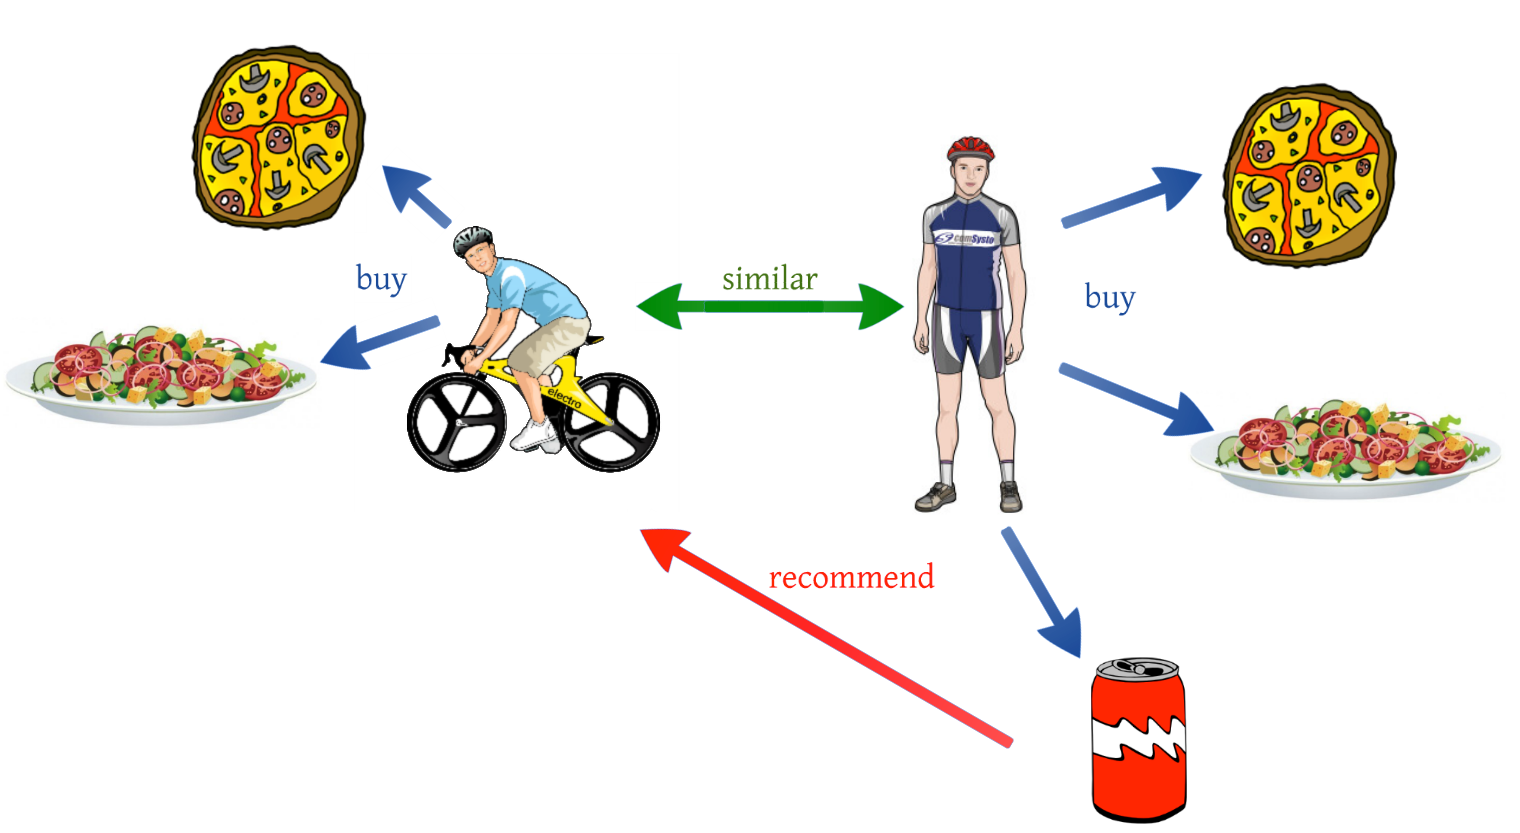
\includegraphics[width=\columnwidth,height=\paperheight,keepaspectratio]{collaborative.png}}
  {\tiny Source: \url{https://medium.com/@akhilesh3091999/recommender-system-bb032b16ab67}}
\end{frame}

\begin{frame}{Item-based filtering}
  \begin{block}{The idea}
    \begin{itemize}[<+>]
      \item If two items are liked by the same users, they are probably similar
      \item We can recommend one item based on the other
    \end{itemize}
  \end{block}
  \begin{exampleblock}{Example}
    Alex, Sanne, and Marthe all like skincare products \textit{X} and \textit{Y}. When Denise buys product \textit{Y}, product \textit{X} is recommended.
  \end{exampleblock}
\end{frame}

\begin{frame}{Item-based filtering: visualised}
  \makebox[\linewidth]{%
    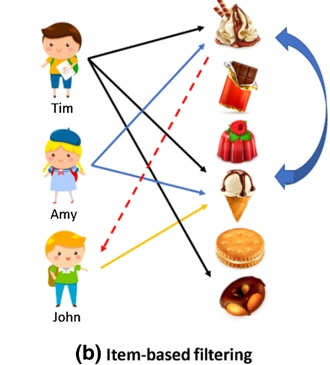
\includegraphics[width=0.5\textwidth]{item_based}}
  {\tiny Source: \url{https://predictivehacks.com/item-based-collaborative-filtering-in-python/}}
\end{frame}

\begin{frame}{Example: Amazon}
  \makebox[\linewidth]{%
    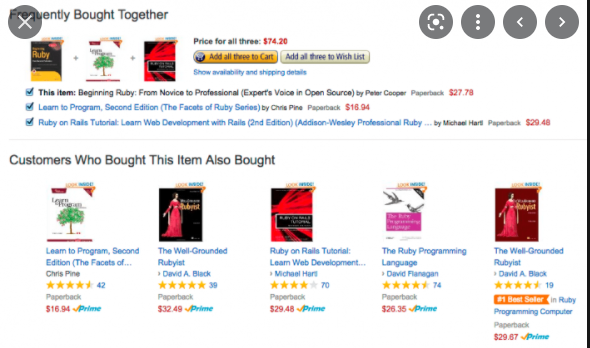
\includegraphics[width=0.5\textwidth]{userbased-amazon}}
\end{frame}

\begin{frame}{Reflection: recommender systems and society}
  \begin{alertblock}{Food for thought}
    \begin{itemize}[<+>]
      \item Recommender systems can have real consequences for democratic values
      \item Filter bubbles, echo chambers, and reduced news diversity are active research topics
      \item As communication scientists, understanding how these systems work is essential
    \end{itemize}
  \end{alertblock}
\end{frame}

\begin{frame}{Big picture: how it all connects}
\centering
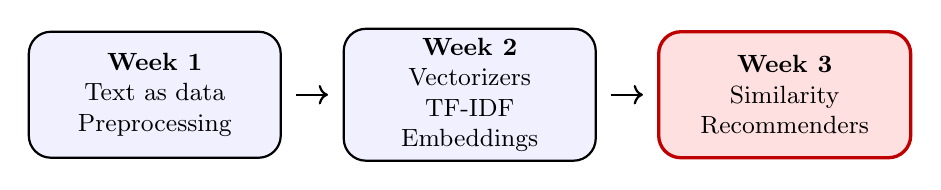
\begin{tikzpicture}[
    every node/.style={font=\small},
    stage/.style={
        draw,
        rounded corners=8pt,
        minimum width=3.2cm,
        minimum height=1.6cm,
        align=center,
        thick,
        fill=blue!6
    },
    highlight/.style={
        draw,
        rounded corners=8pt,
        minimum width=3.2cm,
        minimum height=1.6cm,
        align=center,
        very thick,
        draw=red!75!black,
        fill=red!12
    }
]

\node[stage] (w1) at (0,0) {\textbf{Week 1}\\Text as data\\Preprocessing};
\node[stage] (w2) at (4,0) {\textbf{Week 2}\\Vectorizers\\TF-IDF\\Embeddings};
\node[highlight] (w3) at (8,0) {\textbf{Week 3}\\Similarity\\Recommenders};

\draw[->, thick] (1.8,0) -- (2.2,0);
\draw[->, thick] (5.8,0) -- (6.2,0);

\end{tikzpicture}

\vspace{0.6cm}

\begin{block}{What you learned today}
\begin{itemize}
\item How to compare texts using cosine similarity
\item Why representation affects similarity
\item How similarity is used in recommender systems
\end{itemize}
\end{block}
\end{frame}

\begin{frame}{Key takeaway}
\begin{center}
\Large
Text $\rightarrow$ Representation $\rightarrow$ Similarity $\rightarrow$ Recommendation
\end{center}

\vspace{1cm}

\begin{alertblock}{Core idea}
Change the representation $\rightarrow$ change the similarity $\rightarrow$ change the recommendation
\end{alertblock}

\pause

\begin{block}{Looking ahead}
These ideas are the foundation for:
\begin{itemize}
\item Topic modelling
\item Classification
\item Large-scale text analysis
\end{itemize}
\end{block}
\end{frame}

\begin{frame}{Practice with the materials}
  \begin{exampleblock}{This week's lab session}
    \begin{itemize}[<+>]
      \item Walk through the notebook carefully
      \item Decide whether you want to build a knowledge-based or content-based recommender system
      \item Base your design on the available data columns
    \end{itemize}
  \end{exampleblock}
\end{frame}

\begin{frame}[standout]
  Have fun!
\end{frame}

\begin{frame}[t, allowframebreaks]
  \frametitle{Ref}
  \printbibliography
\end{frame}

\end{document}